%%Nagłówek pliku, konfiguracja stron

\documentclass[12pt,a4paper,oneside]{report} %default 10pt
\usepackage[utf8]{inputenc}
\usepackage{geometry} % to change the page dimensions
\usepackage{booktabs} % for much better looking tables
\usepackage{verbatim} % adds environment for commenting out blocks of text & for better verbatim
\usepackage{float}
\usepackage{amsfonts}
\usepackage{ifpdf}
\usepackage{indentfirst}
\usepackage{fancyhdr} % This should be set AFTER setting up the page geometry
\usepackage[T1]{fontenc}
\usepackage[utf8]{inputenc}
\usepackage[polish]{babel}
\usepackage{caption}
\usepackage{mathtools}

\geometry{a4paper}
\geometry{margin=1in}
\pagestyle{plain}
\renewcommand{\headrulewidth}{0pt}
\lhead{}\chead{}\rhead{}
\lfoot{}\cfoot{\thepage}\rfoot{}
\setlength\parindent{24pt}

\usepackage{listings}
\lstset{literate={ć}{{\'c}}1 {ó}{{\'o}}1 {ś}{{\'s}}1 {ź}{{\'z}}1 {ń}{{\'n}}1
        {Ć}{{\'C}}1 {Ó}{{\'O}}1 {Ś}{{\'S}}1 {Ź}{{\'Z}}1 {Ń}{{\'N}}1
        {ą}{{\k{a}}}1 {ę}{{\k{e}}}1 {Ą}{{\k{A}}}1 {Ę}{{\k{E}}}1 {ż}{{\.z}}1
        {Ż}{{\.Z}}1 {ł}{{\l{}}}1 {Ł}{{\L{}}}1}

\usepackage{color}

\definecolor{dkgreen}{rgb}{0,0.6,0}
\definecolor{gray}{rgb}{0.5,0.5,0.5}
\definecolor{mauve}{rgb}{0.58,0,0.82}

\lstset{frame=tb,
    language=Python,
    aboveskip=3mm,
    belowskip=3mm,
    showstringspaces=false,
    columns=flexible,
    basicstyle={\small\ttfamily},
    numbers=none,
    numberstyle=\tiny\color{gray},
    keywordstyle=\color{blue},
    commentstyle=\color{dkgreen},
    stringstyle=\color{mauve},
    breaklines=true,
    breakatwhitespace=true,
    tabsize=3
}

\title{System doradztwa zawodowego z wykorzystaniem metod sztucznej inteligencji - szkic}
\author{Paweł Tomasik}






%%%%%%%%%%%%%%%%%%%%%%%%%%%%%%%%%%%%%%%%%%%%%%%%%%%%%%%%%%%%%%%%%%%%%%%%%%%
%%Praca właściwa

\begin{document}
\maketitle
%\begin{abstract}
%\title{Słowa kluczowe}
%Python
%\end{abstract}
\renewcommand{\abstractname}{Strzeszczenie}
\begin{abstract}
Praca przedstawia system do przeprowadzania testów doradztwa zawodowego z wykorzystaniem metod analizy danych. Celem przyświecającym temu programowi jest zintegrowanie testów osobowości z technikami analizy danych i uczenia maszynowego. Napisana została aplikacja serwerowa, która umożliwia klientom wzięcie udziału w udostępnionym teście. Wyniki są zapisywane w logu i mogą być wykorzystywane do dalszej analizy. Możliwości narzędzi analitycznych oceniono na podstawie gotowego zestawu danych.
\end{abstract}

\tableofcontents











\chapter{Testy osobowości jako problem analizy danych}

Kwestionariusze są jedną z najbardziej rozpowszechnionych metod badań społecznych. Swoją popularność zawdzięczają przede wszystkim prostocie ich analizy - dane mają najczęściej charakter liczbowy, podlegający mniej lub bardziej, w zależności od metody, narzędziom statystyki.\par

Na znamienną rolę analityki w badaniach społecznych wskazuje istnienie takich platform jak \emph{Survey Monkey} \cite{surveymonkey}, które automatyzują podstawowe testy statystyczne i umożliwiają integrację z zewnętrznymi narzędziami statystycznymi. Natomiast prace takie jak \cite{test-postaw-milosnych} pokazują, że metody sztucznej inteligencji pozwalają udoskonalać metody psychometryczne.\par

Data mining jest nieodłączną częścią procesów przemysłowych związanymi z systemami \emph{Business Intelligence} i \emph{Big Data}. \emph{CRISP-DM} stanowi przemysłowy standard wykorzystywania danych. Jego iteracyjna formuła jest dobrym punktem wyjścia do omówienia procesów związanych z danymi: ich zbieranie, zrozumienie, oczyszczanie, modelowanie i walidację.\par

Celem pracy jest zbudowanie systemu do iteracyjnej budowy i udoskonalania kwestionariuszy i testów osobowości na podstawie odpowiedzi do testu opartego o model RIASEC. W szczególności została wykonana analiza tych danych w celu przygotowania ich do modelowania, zbudowanie systemu do przeprowadzania testów wraz z uzyciem metod klasyfikacji i klasteryzacji oraz udostępnianiem danych do analizy oraz weryfikacja skuteczności użytych klasyfikatorów we wzajemnym porównaniu i w porównaniu do metryki testu.\par










\chapter{Zarys analizy danych}

Analiza danych jest dziedziną zajmującą się procesem wyciągania użytecznej informacji z danych poprzez ich transformację i modelowanie. Natomiast \emph{data mining} jest pojęciem z pogranicza uczenia maszynowego i statystyki. Jest ono różnie definiowanie przez autorów, zjednując je mniej lub bardziej z analizą danych. Niezależnie od definicji, celem obu tych dyscyplin jest odkrywanie wiedzy z danych, przechodzenie od szczegółu do ogółu. Przedstawione definicje wskazują na indukcyjny charakter wnioskowań wypływający z analiz - powstające modele generalizują dane.

Proces analizy składa się z kilku etapów, często nachodzących na siebie i powtarzających się. Poprawna analiza danych musi składać się ze zrozumienia analizowanej próbki, wstępnego przygotowania jej, modelowania i walidacji modelu. 

\section{Techniki eksploracyjnej analizy danych}

Eksploracyjna analiza danych (EDA) stanowi etap przygotowawczy do budowy modelu na danych. Celem EDA jest sformułowanie i wstępne zweryfikowanie przez analityka założeń dotyczących danego problemu na podstawie trendów pojawiających się w próbce. EDA jest wykonywana jako etap poprzedzający confirmatory data analysis. EDA jest też szeroko stosowana jako podstawa do budowania systemów Business Intelligence.\cite{hseltman} \par 

Wykorzystanie technik EDA zależy od rodzaju dostępnych danych oraz od oczekiwanego rodzaju wniosków. Przede wszystkim należy wyróżnić podział na metody \emph{numeryczne} i \emph{wizualne}. Te pierwsze stanowią nieparametryczne metody statystyczne. W szczególności jednak używane są techniki graficzne, pozwalające w łatwy sposób zobrazować kluczowe cechu zestawu danych: trendy, rozrzuty, odstępstwa, rozkłady etc. Techniki różnią się też w zależności od rodzaju danych i wymiarowości, w której operują.\par

Przed przejściem do omówienia poszczególnych technik należy zwrócić uwagę na rodzaje danych. Zgodnie ze \cite{stanisz-1}, wyróznia się cztery \emph{skale} danych: nominalna, porządkowa, równomierna i ilorazowa.. Dane nominalne podlegają jedynie operacji równości i ich analiza jest najbardziej uproszczona. Dla danych porządkowych definiowalne są także relacje nierówności. Dane równomierne i ilorazowe pozwalają na dokładnie określenie odległości między punktami, przy czym dla skali ilorazowej da się określić punkt zerowy. (citation needed)\par

\subsection{Metody numeryczne}

Podstawą do analizy danych jest zestawienie próbki w postaci szeregu. W przypadku uszeregowania danych względem jakiejś zmiennej mówi się o szeregu szczegółowym. W opisanym zastosowaniu o wiele bardziej interesujący jest szereg rozdzielczy, który grupuje dane na klasy i zlicza ilośc wystąpień w danej klasie. Jest to szczególnie przydatne w przedstawianiu wyników klasteryzacji zbioru danych. \par

Podstawą dla statystyki są cztery wielkości, które opisują daną próbkę. Dane można opisywać wielkościami opisującymi centrowanie(lokację), zmienność, asymetrię i koncentrację. \cite{stanisz-1} Metody opisujące dane nominalne różnią się od metod ilościowych. Przede wszystkim dla danych nominalnych lub porządkowych nie można określić rozkładu prawdopodobieństwa. Miary tych wielkości dla dwu rodzajów danych zestawiono w tabeli \ref{miary-statystyczne} 

\begin{table}
\begin{tabular}
Wielkość & Miara porządkowa & Miara równomierna  \\
Wyśrodkowanie & Mediana, mediana ważona, moda & Średnia, średnia ważona \\
Zmienność & Rozstęp, rozstęp międzykwartylowy & Wariancja, wariancja ważonam odchylenie standardowe \\
Asymetria &  & współczynnik skośności \\
koncentracja &  & kurtoza \\
\end{tabular}
\caption{Zestawienie wielkości opisujących próbkę}
\label{miary-statystyczne}
\end{table}

Miarą \emph{lokacji} jest w tym przypadku mediana lub moda. \emph{Mediana} jest środkową wartością dla uporządkowanego szeregu pomiarów. \emph{Moda} lub \emph{dominanta} to wartość najczęściej w zbiorze występująca. \emph{Pierwszy i trzeci kwartyl} to punkty leżące odpowiednio w 1/4 i 3/4 uporządkowanego szeregu. Miarami \emph{rozrzutu} są \emph{rozstęp} i \emph{rozstęp ćwiartkowy}, zdefiniowane jako różnice odpowiednio skrajnych wartości i wartości kwartyli. \par

\subsection{Metody wizualne}

Zgodnie z \cite{nist} metody wizualne stanowią wyróżnik eksploracyjnej analizy danych nad statystycznym podejściem do formułowania hipotez. W istocie metody wizualne w o wiele większym stopniu polegają na intuicji analityka niż na systematycznym podejściu. Rozmaite techniki wykreślania danych przedstawiono na zestawieniach takich jak \cite{visual-literacy} czy \cite{viz-catalogue}. Opisane zostaną tutaj tylko techniki wykorzystane w realizacji projektu. \par

Wykresy dla nieprzetworzonych danych (\emph{raw data}) to między innymi histogramy i bihistogramy, wykresy typu \emph{box and whiskers} czy wykresy bąbelkowe. Pierwsze dwa stosowane są do ukazania podstawowych danych o częstotliwościach występowania cechy w próbce, a ostatni do zestawiania dwóch cech. \par

Wykresy dla danych przetworzonych to wykresy biegunowe lub gwiazdowe (\emph{polar chart, star plot}), które pozwalają zestawić wszystkie cechy danej kategorii na jednym obrazie, a ich złożenie pozwala porównać między soba poszczególne kategorie. \par

\section{Wstępne przetwarzanie danych}

Modele statystyczne wykorzystywane w analityce w większości przypadków nie są przygotowane by radzić sobie z niepoprawnymi lub niekompletnymi danymi. Z tego powodu po zrozumieniu próbki wykonuje się etap oczyszczania i przygotowania danych. \par

\subsection{Usunięcie elementów odstających}

Jednym z zadań EDA jest \emph{wykrywanie obserwacji odstających}. Ma ono na celu wyeliminowanie elementów, które znacznie różnią się od przeciętnego pomiaru w wyniku bądź to błędu pomiaru, celowego zniekształcenia lub rzeczywiście nietypowych indywiduów. O ile wyeliminowanie ostatnich może prowadzić do błędu klasyfikatora, o tyle w większości przypadków właśnie pozostawienie anomalii, jak się te pomiary czasem nazywa, powoduje większe obniżenie jakości modelu. \cite{dudek} \par

\subsection{Redukcja wymiarowości}

Jednym z celów zastosowania EDA do tej aplikacji jest zredukowanie ilości pytań dla każdego z testów. Ograniczenie ilości pytań w modelu bierze się z dwóch przyczyn. Pierwszą z nich jest wygoda użytkownika - z założenia osoba biorąca udział w teście zawodowym nie jest skłonna wypełniać bardzo długich kwestionariuszy.\par

Druga cecha związana jest z dopasowaniem modeli do dużych zestawów danych. \emph{Curse of dimensionality} jest pojęciem związanym z uczeniem maszynowym i ogólnie pojętą analityką, opisujące postępujące rozrzedzenie danych w miarę wzrostu ich wymiarowości. (czy jest to prawda - źródła poddają w wątpliwość)\par

\subsection{Nadmierne dopasowanie}

Zjawisko nadmiernego dopasowania, czy też overfittingu jest czynnikiem nakładającym górną granicę na ilość próbek dostarczanych do modelu. Dla dziedziny $X$ hipoteza $h$ jest nadmiernie dopasowana, gdy istnieje hipoteza h' o większym błędzie próbki a mniejszym rzeczywistym.\par

Nadmiernie dopasowana hipoteza oddaje przekłamania na danych. Ponadto, hipotezy zbyt dopasowane są porównywalne do interpolacji zaszumionych danych - po prostu zniekształcają obraz rzeczywistości. innymi słowy - bardziej trafne mogą być hipotezy niespójne na danych wejściowych.\par
















\section{Uczenie maszynowe}

Uczenie maszynowe (\emph{machine learning}) stanowi jeden z ostatnich trendów technologicznych. Jest też identyfikowany przez Gartnera jako jedna z najbardziej przecenianych technologii w obecnej nauce \ref{gartner}. Bądź co bądź, odpowiednio wykorzystane techniki ML są z powodzeniem stosowane w takich technologiach jak modelowanie zużycia energii, rozpoznawanie emocji, identyfikacja obiektów na zdjęciach, systemy \emph{speech-to-text} i wiele innych. Wystarczy przyjrzeć się najnowszym dokonaniom firm takich jak Amazon, Microsoft aby przekonać się, że powstała szeroka gama usług opartych o \emph{soft computing}, z uczeniem maszynowym na czele. \par

\begin{figure}
\caption{\emph{Hype cycle} Gartnera, rok 2016}
\centering
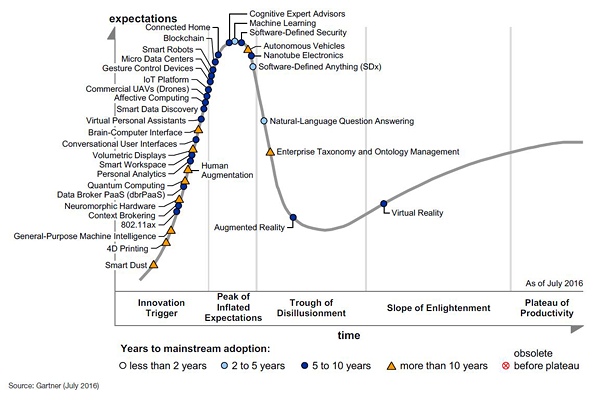
\includegraphics[width=0.5\textwidth]{gartner.png}
\label{gartner}
\end{figure}

Z punktu widzenia analizy danych, uczenie maszynowe jest sposobem na budowę modelu na danych. W istocie klasyfikatory typu bayesowskiego są niczym innym jak praktycznym zastosowaniem reguł prawdopodobieństwa. Zaletą uczenia maszynowego jet automatyczne budowanie hipotezy na danych w przeciwieństwie do klasycznego wnioskowania statystycznego, które wymaga od analityka postawienia hipotez do weryfikacji. \par

"Uczeniem się systemu jest każda autonomiczna zmiana w systemie zachodząca na podstawie doświadczeń, która prowadzi do poprawy jakości jego działania"\cite{cichosz}. Podstawowym celem uczenia maszynowego jest przeprowadzenie \emph{wnioskowania}. Wnioskowanie w rachunku zdań potraktować jako trójkę $ P \and W \rightarrow K $, co oznacza, że przesłanki oraz wiedza implikują konkluzję. Wnioskowanie dzieli się na indukcyjne i dedukcyjne. \par

Wnioskowanie indukcyjne stanowią metody wyciągające ogół ze szczegółu, generalizujące dane do postaci wiedzy. Przykładem jest formowanie reguł podziału na grupy w oparciu o zestaw danych treningowych. Wnioskowanie dedukcyjne stanowi zaaplikowanie wiedzy do określonej sytuacji - w tym wypadku byłoby to użycie tych reguł do nowych danych. \par

W niniejszej pracy przedstawione są dwa z trzech zasadniczych problemów data miningu: klasyfikacja oraz klasteryzacja. Zarówno problem klasyfikacji i klasteryzacji definiuje się w podobny sposób: istotą problemu jest przydzielenie każdego elementu ze skończonego zbioru \emph{obiektów} do jednej lub kilku grup zwanych \emph{kategoriami}. \par

Klasyfikacja może być rozumiana jako uczenie pojęć. Mając zestaw par dane-oczekiwany wynik, możemy określić tę metodę jako \emph{uczenie z nadzorem}. Celem algorytmu klasyfikujacego jest znalezienie takiej hipotezy, która najlepiej opisuje zależność między przesłanką a konkluzją. W konkretnych zastosowaniach przesłanką jest najczęściej zbiór cech danego obiektu, konkluzją zaś przynależność jego do pewnej klasy obiektów, stąd też nazwa problemu. \par

Grupowanie(clustering) to zadanie tworzenia pojęć bez uprzedniej wiedzy, co klasyfikuje je jako problem \emph{uczenia bez nadzoru}. Możliwe jest rozbicie problemu na dwa zadania: podział na grupy i naukę pojęć. Zazwyczaj realizuje to jedna metoda (kmeans na przykład), jednak można te dwa zadania rozdzielić - wtedy algorytm grupujący generuje dane do algorytmu klasyfikującego.\par

Aby podział na kategorie był satysfakcjonujący, musi spełniać dwa kryteria. Po pierwsze, elementy wewnątrz kategorii muszą być mozliwie do siebie podobne. Po drugie, elementy z różnych kategorii muszą różnić się od siebie o ile jest to tylko możliwe.\par

Aby możliwe było opisanie problemu, potrzebna jest formalne zdefiniowanie zarówno cech, jak i podobieństwa. W praktyce cechy można definiować dwojako: jako wartości binarne lub rzeczywiste (znormalzowane do jedności, lub nie). W ten sposób opis danego obiektu przyjmuje postać wektora cech (ang. \emph{features}). W takiej reprezentacji miarą podobieństwa, lub bardziej niepodobieństwa, jest odległość między tymi dwoma wektorami. Formalnie podobieństwo $s$ definiuje się jako:\par

\begin{equation}
tu-wzor
\end{equation}

Ważnym pojęciem do zmierzenia podobieństwa między dwoma obiektami jest pojęcie \emph{metryki}. Metryka jest funkcją, która przyjmując dwa wektory zwraca odległość między nimi. O ile pojęcie odległości pojmowane intuicyjnie jest jednoznaczne, jednak dla celów rozróżnienia obiektów, które są wektorami w przestrzeni o bardzo wielu wymiarach, odpowiednio dobrana metryka pozwala na lepsze dopasowanie modelu klasy do rzeczywistego rozkładu cech wśród jej członków.\par

Najważniejsze dwie metryki to metryka euklidesowa, oraz metryka Manhattan. Są one rozszerzeniem ogólnej metryki Minkowskiego, podanej we wzorze (?). Szczególnym przypadkiem metryki typu Manhattan jest metryka Hamminga, która dla ciągów binarnych jest analogiem sumą bitów jedynkowych funkcji XOR. \par

Drugim elementem, poza metryką, definiującym kształt klasy jest \emph{norma}. Norma ma najczęściej postać macierzy $n \times n$ współczynników, gdzie $n$ to długość wektora cech, w której znajdują się współczynniki przekształcające wektor w taki sposób, aby zrównoważyć wpływ różnego rozrzutu cech na klasyfikację, jak i uwzględnić zależności między cechami. \par

Uzbrojeni w definicję podobieństwa i sposób jego obliczenia, jesteśmy w stanie w miarę dobrze ocenić poprawność działania algorytmów. Ważnym elementem różnych rozwiązań jest też sposób klasyfikacji: dzieli się ją na \emph{ostrą}, \emph{rozmytą} i \emph{posybilistyczną}. Klasyfikacja ostra przyporządkowuje obiekt do jednej i tylko jednej klasy. Klasyfikacja rozmyta wiąże obiekt z róznymi klasami z różną siłą, przy czym suma współczynników określających przynależność dla danego obiektu jest zawsze równa jedności. Klasifykacja posybilistyczna różni się od poprzedniej zniesieniem ograniczenia sumy.\par

\subsection{Naiwny klasyfikator bayesowski}

Jedna z prostszych metod klasyfikacji opiera się na definicji prawdopodobieństwa warunkowego, zwanej także regułą Bayesa. Stanowi ona związek między prawdopodobieństwami dwóch zmiennych oraz prawdopodobieństwami implikacji jednej zmiennej z drugiej i vice versa. Pozwala ona obliczać prawdopodobieństwo implikacji odwrotnej do implikacji podanej w danych. Reguła ma następującą postać:

\begin{equation}
P(C|\vec{x}) = \frac{P(\vec{x}|C)P(C)}{P(\vec{x})}
\end{equation}

Prawdopodobieństwo złożonej zmiennej $\vec{x}$ jest równe iloczynowi prawdopodobieństw jego składowych, jak pokazano we wzorze \ref{pp-zlozone}. Analogicznie można otrzymać prawdopodobieństwo złożonej implikacji \ref{pp-implikacji} (citation needed). Obydwa wzory funkcjonują na założeniu \emph{niezależności} zmiennych, mianowicie prawdopodobieństwo jednej zmiennej nie jest zależne od żadnej innej. \ref{niezaleznosc}. "Naiwność" klasyfikatora wynika właśnie z założenia niezależności zmiennych, co nie zawsze jest prawdą. Uwzględnienie zależności zmiennych pozwala tworzyć kaskadowe modele zwane sieciami bayesowskimi.\cite{dm-cichosz} Nie są one jednak częścią tej pracy.\par

\begin{equation}
P(\vec{x}) = \prod{P(x_i)}
\end{equation}
\label{pp-zlozone}

\begin{equation}
??
\end{equation}
\label{pp-implikacji}

\begin{equation}
??
\end{equation}
\label{niezaleznosc}

Naiwny klasifykator bayesowski dla danego wektora wejściowego $\vec{x}$ testuje prawdopodobieństwo każdej z hipotez $P(C_j|\vec{x}) | C_j \in C$, gdzie C to zbiór zdarzeń elementarnych polegających na przynależności elementu do jednej z kategorii. W przypadku klasyfikacji ostrej $\sum_{C_j \in C} P(C_j) = 1 $. Za prawdopodobieństwa zdarzeń elementarnych wchodzących w skład reguły Bayesa przyjmuje się prawdopodobieństwa wystąpienia danych zdarzeń w próbce uczącej. \par

Ze względu na fakt, iż dla nie występującego w próbce uczącej wektora $P(\vec{x}) = 0$ oraz fakt, że $P(\vec{x})=const$ dla każdego $C_j$ człon pomija się, uzywając do klasyfikacji miary proporcjonalnej do prawdopodobieństwa. Następnie jako wynik klasyfikacji przyjmuje się zdarzenie, które osiąga najwyższą miarę.\par

\emph{Wady i zalety Kl.B}
Wady:
mała akceptowalna ilość hipotez(klasyfikator bierze pod uwagę wszystkie hipotezy i nimi operuje)
nieuwzględnienie uporządkowania kategorii (a więc trzeba wstępnie wyznaczyć pojęcia)
Zalety:
O(n)

\emph{a priori i a posteriori}

\subsection{Klasyfikator maksymalnoogległościowy}

Klasyfikatory maksymalnoodległościowe zostały wynalezione przez Vapnika. Opierają się one na wyznaczeniu granicy między zestawmi danych w taki sposób, aby zachować możliwie dużą odległość najbliższych punktów od granicy. Inna nazwa tej metody, \emph{maszyna wektorów wspierających}, oddaje sposób w jaki zostaje to wykonane. Wybiera się $n$ punktów:\par
... opis działania metody...\par
Istotne do poprawnego wykorzystania SVM jest wykonanie kilku kroków \cite{chih-wei}. Po pierwsze, należy przygotować i znormalizować dane. Drugim etapem jest wybór rodzaju funkcji jądra. Standardowo rozróżnia się cztery jej rodzaje: liniowe, wielomianowe, RBF i sigmoidalne. Następnie, należy ocenić odpowiednio \emph{ten parametr jądra}. Zgodnie z badaniami samego autora tej metody, musi być on równy wymiarowi $VC$ (\emph{Vapnika-Chernocośtam}) dla zbioru danych. Wymiar VC definiuje się w sposób podany we wzorze \ref{wymiar-vc}. Wraz z oceną tego parametru należy jeszcze znaleźć współczynnik błędu. \par

\begin{equation}
VC(x) = max(d) => d różnych przykładów w dziedzinie X podzielone na wszystkie 2^d możliwych sposobów (dla binarnego zaklasyfikowania)
\end{equation}
\label{wymiar-vc}

\subsection{Metoda k średnich}

Metoda k-średnich stanowi niewątpliwie jeden z najprostszych algorytmów klasyfikujących. Jej działanie opiera się na iteracyjnym grupowaniu i klasyfikowaniu elementów. Jego działanie najlepiej przedstawione jest na rysunku \ref{kmeans-png}. Cykl poprawiania średnich trwa aż ich zmiana będzie mniejsza od progu.

\begin{figure}
\caption{\emph{Hype cycle} Gartnera, rok 2016}
\centering
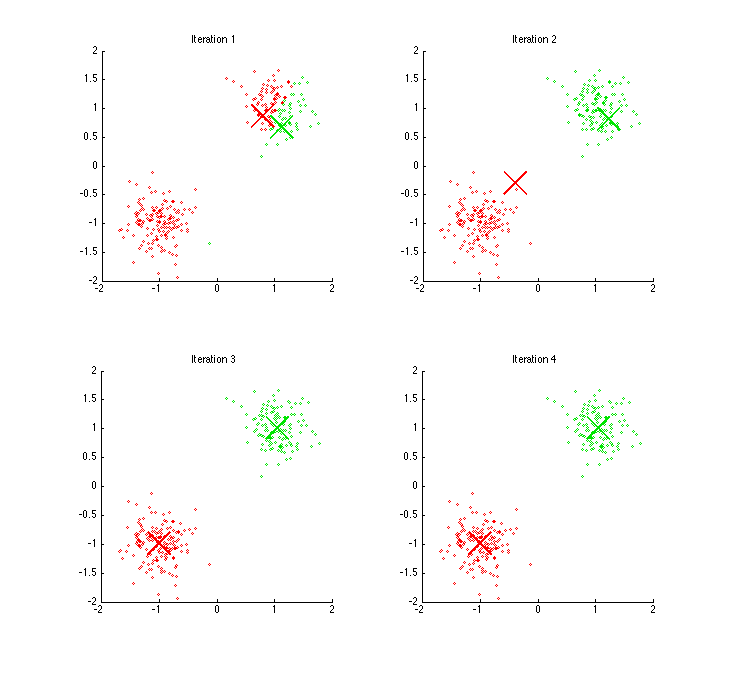
\includegraphics[width=0.5\textwidth]{kmeans.png}
\label{kmeans-png}
\end{figure}

O ile algorytm jest bardzo prosty w implementacji, o tyle posiada szereg wad: po pierwsze, liczba kategorii musi być odgórnie znana. Po drugie, algorytm działa w miarę dobrze jedynie dla danych o wyraźnie zarysowanych granicach. Kolejną sprawą, którą należy mieć na uwadze jest NP-złożoność, co sprawia, że algorytm staje się niewygodny dla duzych zestawów danych.




\section{Walidacja}



\subsection{Walidacja krzyżowa}

Błąd próbki:
$    e_P^c(h) = \frac{| \{ x \in P | h(x) != c(x) \} |}{|P|} $
Liczba pomyłek:
$        r_P^c(h) = | \{ x \in P | h(x) != c(x) \} | $
Błąd rzeczywisty:
$    e_\Omega^c (h) = Pr_{x \in \Omega}(h(x) != c(x))$ gdzie Omega to rozkład prawdopodobieństa
Możemy przypisać $\Omega$ jako jednorodnemu rozkładowi spośród próbki danych weryfikacyjnych
            
            





\chapter{Opis wykorzystanego kwestionariusza}

Do zrealizowania systemu wybrano ogólnodostępny zestaw danych psychologicznych, pobrany ze strony internetowej \ref{raw_data}. Dane zawierają wyniki testu przeprowadzonego w Internecie wraz z metryczką demograficzną. Test składa się z 48 pytań w pięciostopniowej skali Likerta.

\section{Model Hollanda}

Model ten opracowany przez John'a Hollanda w roku 1959. \cite{holland-source} Klasyfikuje on ludzi na sześć głównych klas, a bardziej szczegółowo, szereguje funkcje zawodowe ludzi według ich preferencji. Te sześć funkcji zestawionych jest w przeciwstawne pary:\par
Artystyczny - Konwencjonalny\par
Realistyczny - Spoleczny\par
Badawczy - Przedsiebiorczy\par
Zawody są przydzielone do jednej lub kilku z tych klas według umiejętności, których wymagają, mogą one należeć także do klas przeciwstawnych, jeżeli obydwie umiejętności są potrzebne - nie wykluczają się one wzajemnie.\par

\emph{identity,diversity and other - base on the citation}

\section{Skala Likerta}

Skala Likerta jest techniką psychometryczną używaną w celu zmierzenia stopnia zgodności respondenta z danym poglądem lub podejściem. Skala ta najczęściej jest jednowymiarowa. Składa się z małej ilości odpowiedzi przedstawiąjach symetrycznie ułożone punkty na osi \emph{zgodność}-\emph{niezgodność}, w nieparzystej ilości(zazwyczaj 5). \cite{bertram}

Założenie, że punkty przedstawiają równoodległe natężenia cechy, pozwala traktować skalę jako źródło danych interwałowych. Dane interwałowe oddają różnice między różnymi poziomami danej cechy, nie określają jednak jej absolutnej wartości (punktu zerowego)  \cite{bertram}

Analiza wyników testu opartego na tej skali zależy od sposobu ujęcia odpowiedzi. Jeżeli analizujemy pojedyńcze zdania, danych nie można traktować jako danych interwałowych i stosuje się wtedy techniki nieparametryczne. Natomiast wziąwszy zestawy odpowiedzi opisujące poszczególną cechę, można potraktować tę technikę jako metodę ilościową i stosować metody statystyki parametrycznej. \cite{joe} Z tego też powodu skala Likerta zwana jest także techniką sumacyjną

\emph{Jak potraktować skalę Likerta}









\chapter{Implementacja}

W ramach pracy zbudowany został system pozwalający przeprowadzać testy na podstawie kwestionariuszy, przeprowadzać klasyfikację respondentów na podstawie odpowiedzi i analizować zebrane dane. Aplikacja została napisana w języku Python, który jest szeroko wykorzystywany w środowiskach analitycznych. Wykorzystano wersję języka o numerze 2.7.

Front-end aplikacji, który stanowi także jej szkielet, napisano przy pomocy pakietu \emph{Flask}. Jest to open-source'owy lekki serwer HTTP, wykorzystujący język pomocniczy \emph{Jinja2} do generacji dokumentów HTML przy pomocy danych z aplikacji. Mechanizm ten użyty został do wstrzykiwania danych testu do prostej aplikacji sieciowej opartej o \emph{Javascript}. Użytkownik może wybrać test na stronie głównej, można też udostępniać testy jedynie przy pomocy statycznych linków.

Test generowany przez aplikację może zawierać pytania o charakterze binarnym, jak i przy użyciu skali \emph{likert}. Podczas przebiegu testu ukazywane jest tylko jedno pytanie na raz, co pozwala skupić się na odpowiedzi. Wyniki są zbierane dopiero w przypadku ukończenia testu. Po zakończonym teście użytkownik jest przekierowywany na stronę, na której może udostępnić dodatkowe informacje w celach analityki. Po przejściu tego etapu wyświetlany jest raport z testu.

Generacja raportów oparta jest o pakiety \emph{pandas} oraz \emph{matplotlib}. Użycie tych dwóch bibliotek pozwala na używanie najpowszechniejszych metod analityki na zestawach danych, włącznie z generowaniem wykresów. Struktura raportów oparta jest o definicje w plikach konfiguracyjnych poszczególnych testów(o których później). Zawierają one definicje raportów zbudowane przy użyciu struktury przypominającej struktury języka LISP, używające składni JSON.

Metody klasyfikacji oraz uczenia maszynowego pochodzą z biblioteki \emph{sklearn}. Są one udostępniane jako dyrektywy do języka konfiguracyjnego. Istnieje możliwość nauczenia klasyfikatorów w trakcie uruchamiania aplikacji, jak i ich dynamiczne zastępowanie nowymi w trakcie działania aplikacji. Wykorzystane techniki obejmują: klasifykator Bayesowski, metodę k-średnich

Aplikacja udostępnia widok, który generuje raporty dla całego zestawu danych. Raporty te mogą korzystać z danych wzorcowych jak i zebranych podczas testowania. Funkcja ta ma na celu umożliwienie przeprowadzenia analizy danych, zarówno wstępnej jak i weryfikacyjnej, która z kolei umożliwi dopracowanie modelu.

Front-end udostępnia także widok interaktywny do budowania raportów z danych bez wcześniejszego definiowania ich. Użyty jest ten sam język, co w plikach konfiguracji raportów. Pozwala to na sprawdzanie hipotez bez konieczności rebootowania aplikacji.

\section{Pliki konfiguracyjne}

Pliki konfiguracyjne do programu oparte są o standard JSON. Pozwala to na łatwe wbudowanie złożonych ustawień takich jak sekwencje wykonywanych operacji podczas generowania odpowiedzi na test czy precyzowanie pytań o różnej strukturze.

Głównym plikiem konfiguracyjnym jest \texttt{static/tests.json}. W nim zawarte są informacje dotyczące: zestawu pytań, lokalizacji logów i danych odniesienia, dodatkowych parametrów testu oraz metod generacji raportów. Kompletną listę dyrektyw zestawiono w tabeli \texttt{reporting-lang}. Drugim typem plików konfiguracyjnych są pliki linkowane przez poszczególne testy. Struktura takiego pliku to lista obiektów przedstawiających pytania do testów.

Schemy tych dwóch rodzajów plików przedstawione są w tabelach \ref{tests-schema} i \ref{questions-schema}

\section{Instalacja i uruchomienie}

Całość programu zaopatrzono w skrypty instalacyjne do generacji niezależnego środowiska Pythona \emph{virtualenv}. Ze względu na trudności związane z domyślną lokalizacją biblioteki \emph{libsvm}, która jest związana z zewnętrznym plikiem wykonywalnym napisanym w C, postanowiono uruchamiać ten program poprzez powłokę systemu i komunikować się przy pomocy plików tymczasowych. Aplikację udostępniono na chmurze Amazona pod adresem IP \emph{54.93.169.189}(stan na 30 listopada 2016r.). Kod źródłowy wraz z tekstem tej pracy i notatkami udostępniono poprzez serwis github: \emph{https://github.com/Zantyr/dissertation}\par










\chapter{Wyniki analiz i przedstawienie działania aplikacji}
\section{Wyniki EDA}
\section{Porównanie trafności klasyfikatorów}
\section{Wnioski wyciągnięte z badań}











\chapter{Kod źródłowy}
Poniżej wypisano wszystkie pliki używane w aplikacji do jej konstrukcji. Aplikacja działa pod systemami \emph{Linux Mint} oraz \emph{Linux Ubuntu}, aczkolwiek powinna działać na każdym systemie bazowanym na dystrybucji \emph{Debian}. Wszystkie pliki wykorzystują kodowanie UTF-8.
\section{Wsadowy skrypt instalacyjny (Unix)}
%\lstinputlisting[breaklines]{src/install.sh}
%\lstinputlisting[breaklines]{src/run.sh}
\section{Kod serwera i udostępniane widoki}
%\lstinputlisting[breaklines]{src/main.py}
%\lstinputlisting[breaklines]{src/templates/added.html}
%\lstinputlisting[breaklines]{src/templates/console.html}
%\lstinputlisting[breaklines]{src/templates/main.html}
%\lstinputlisting[breaklines]{src/templates/pick.html}
%\lstinputlisting[breaklines]{src/templates/quiz.html}
%\lstinputlisting[breaklines]{src/templates/report.html}
%\lstinputlisting[breaklines]{src/templates/result.html}
\section{Kod modułów analitycznych}
\section{Pozostałe pliki}

\begin{thebibliography}{9}
\bibitem{test-postaw-milosnych} Roguski K. \emph{Zastosowanie sztucznych sieci neuronowych w psychologicznej analizie osobowości na przykładzie metod psychometrycznych. Praca dyplomowa magisterska}, Wydział Elektryczny Politechniki Warszawskiej, Warszawa 2004
\bibitem{cichosz} Paweł Cichosz, \emph{Systemy uczące się}
\bibitem{dm-cichosz} Paweł Cichosz, \emph{Data Mining Algorithms}
\bibitem{flasinski} Mariusz Flasiński, \emph{Wstęp do sztucznej inteligencji}
\bibitem{raw-data} \emph{http://personality-testing.info/_rawdata/}
\bibitem{hseltman} \emph{Experimental Design and Analysis, http://www.stat.cmu.edu/~hseltman/309/Book/Book.pdf}
\bibitem{bertram} Bertram Dane, \emph{Likert Scales} http://poincare.matf.bg.ac.rs/~kristina/topic-dane-likert.pdf
\bibitem{joe}   https://www.joe.org/joe/2012april/pdf/JOE_v50_2tt2.pdf
\bibitem{holland-source} http://www.counseling.org/docs/david-kaplan's-files/nauta.pdf?sfvrsn=2
\bibitem{dudek} \emph{http://www.gdudek.el.pcz.pl/files/SUS/SUS_wyklad15.pdf}
\bibitem{nist} \emph{http://www.itl.nist.gov/div898/handbook/eda/section3/eda3.htm}
\bibitem{visual-literacy} \emph{http://www.visual-literacy.org/periodic_table/periodic_table.html}
\bibitem{viz-catalogue} \emph{http://www.datavizcatalogue.com/}
\end{thebibliography}
\end{document}
